\documentclass[10pt]{beamer}

\usetheme[progressbar=foot]{metropolis}
\usepackage{appendixnumberbeamer}

\usepackage{booktabs}
\usepackage[scale=2]{ccicons}

\usepackage{pgfplots}
\usepgfplotslibrary{dateplot}
\pgfplotsset{compat=1.18} 

\usepackage{xspace}
\usepackage{xcolor}

\DeclareMathOperator{\stdev}{stdev}
\DeclareMathOperator{\var}{var}
\DeclareMathOperator{\cov}{cov}
\DeclareMathOperator{\corr}{corr}
\DeclareMathOperator{\prob}{prob}
\DeclareMathOperator{\n}{n}
\DeclareMathOperator{\N}{N}
\DeclareMathOperator{\Cov}{Cov}

\newcommand{\hlf}{\frac{1}{2}}
\newcommand{\bi}{\begin{itemize}}
\newcommand{\ei}{\end{itemize}}
\newcommand{\im}{\item}
\newcommand{\D}{\mathrm{d}}
\newcommand{\E}{\mathrm{e}}
\newcommand{\mye}{\ensuremath{\mathsf{E}}}
\newcommand{\myreal}{\ensuremath{\mathbb{R}}}
\newcommand{\bq}{\begin{equation}}
\newcommand{\eq}{\end{equation}}
\newcommand{\eqdef}{\;\buildrel \text{d{}ef}\over = \;}
\newcommand{\xstar}{\buildrel *\over X}
\newcommand{\pmax}{p^{\text{max}}}
\newcommand{\qmax}{q^{\text{max}}}
\newcommand{\bfr}{\begin{frame}}
\newcommand{\bfrp}{\begin{frame}[plain]}
\newcommand{\efr}{\end{frame}}
\newcommand{\F}{\mathcal{F}}
\newcommand{\FF}{\mathbb{F}}
\newcommand{\ve}{\varepsilon}
\newcommand{\lh}{\hat{\lambda}}
\definecolor{mycolor}{gray}{0.8}
\definecolor{mymaincolor}{rgb}{0.6862745098039216,0.9333333333333333,0.9333333333333333}
\newcommand{\alr}[1]{\textcolor{blue}{#1}}
\definecolor{LightCyan}{rgb}{0.88,1,1}
\newcommand{\yel}{\cellcolor{yellow}}
\newcommand{\blue}{\cellcolor{SkyBlue}}
\newcommand{\gr}{\cellcolor{SpringGreen}}
\newcommand{\pink}{\cellcolor{pink}}
\newcommand{\apr}{\cellcolor{Apricot}}
\newcommand{\tve}{\tilde{\varepsilon}}
\newcommand{\tw}{\tilde{w}}
\newcommand{\ttth}{\tilde{\theta}}
\newcommand{\te}{\tilde{e}}
\newcommand{\ts}{\tilde{s}}
\newcommand{\tx}{\tilde{x}}
\newcommand{\ty}{\tilde{y}}
\newcommand{\tv}{\tilde{v}}
\newcommand{\tp}{\tilde{p}}
\newcommand{\tF}{\tilde{F}}
\newcommand{\tf}{\tilde{f}}
\newcommand{\tZ}{\tilde{Z}}
\newcommand{\ow}{\overline{w}}
\newcommand{\tm}{\tilde{m}}
\newcommand{\tc}{\tilde{c}}
\newcommand{\tz}{\tilde{z}}
\newcommand{\tr}{\widetilde{R}}
\newcommand{\tR}{\widetilde{\mathbf{R}}}
\newcommand{\bms}{\begin{multline*}}
\newcommand{\ems}{\end{multline*}}
\newcommand{\bas}{\begin{align*}}
\newcommand{\eas}{\end{align*}}
\newcommand{\qr}{\mathbb{Q}}
\newcommand{\tX}{\tilde{X}}
\newcommand{\tY}{\tilde{Y}}

\setbeamertemplate{frame footer}{BUSI 521/ECON 505, Spring 2024}

\title{Chapter 5: Mean-Variance Analysis}

\date{}
\author{Kerry Back\\ 
BUSI 521/ECON 505\\
Rice University}


\begin{document}

\maketitle
  
  
  \section{Standard Deviation -- Mean Plots}\subsection{}
  
  \bfr\frametitle{Notation}
  \bi
  \im $n$ risky assets with returns $\tr_i$.  $\tR = (\tr_1 \cdots \tr_n)'$
  \im $\mu=\,$ vector of expected returns.  At least two of the assets have different expected returns.
  \im  $\Sigma =\,$ covariance matrix. Assume no redundant assets, so $\Sigma$ is positive definite.
  \im $\iota=\,$ $n$--vector of 1's.
  \im $\pi \in \myreal^n$ is a portfolio (of risky assets).  If the portfolio is fully invested in risky assets, then $\iota'\pi=1$.  Otherwise, $1-\iota'\pi$ is the fraction of wealth invested in the risk-free asset.
  \ei
  \end{frame}
  
  
  \bfr\frametitle{Portfolio Mean and Standard Deviation}
  \bi
  \im Two assets with expected returns $\mu_i$, standard deviations $\sigma_i$, and correlation $\rho$. 
  \im Portfolio $(\pi_1, \pi_2)$ with $\pi_1+\pi_2=1$.
  \im Portfolio return is 
  $$\pi' \tR \ = \ \pi_1\tilde{R}_1 + \pi_2\tilde{R}_2 $$
   \im Portfolio expected return is 
  $$\pi'\mu \ = \ \pi_1\mu_1 + \pi_2\mu_2 $$
  \im Write the covariance matrix as
  $$\Sigma \ = \ \begin{pmatrix} \sigma_1^2 & \rho\sigma_1\sigma_2 \\ \rho\sigma_1\sigma_2 & \sigma_2^2
  \end{pmatrix}$$
   \im The portfolio variance is
  $$\pi'\Sigma\pi \ = \ \pi_1^2\sigma_1^2 + \pi_2^2\sigma_2^2 + 2\pi_1\pi_2\rho\sigma_1\sigma_2$$
  \ei
\end{frame}
  
  \bfr\frametitle{Portfolios of Two Risky Assets}
  \vskip -\baselineskip
  \begin{center}
  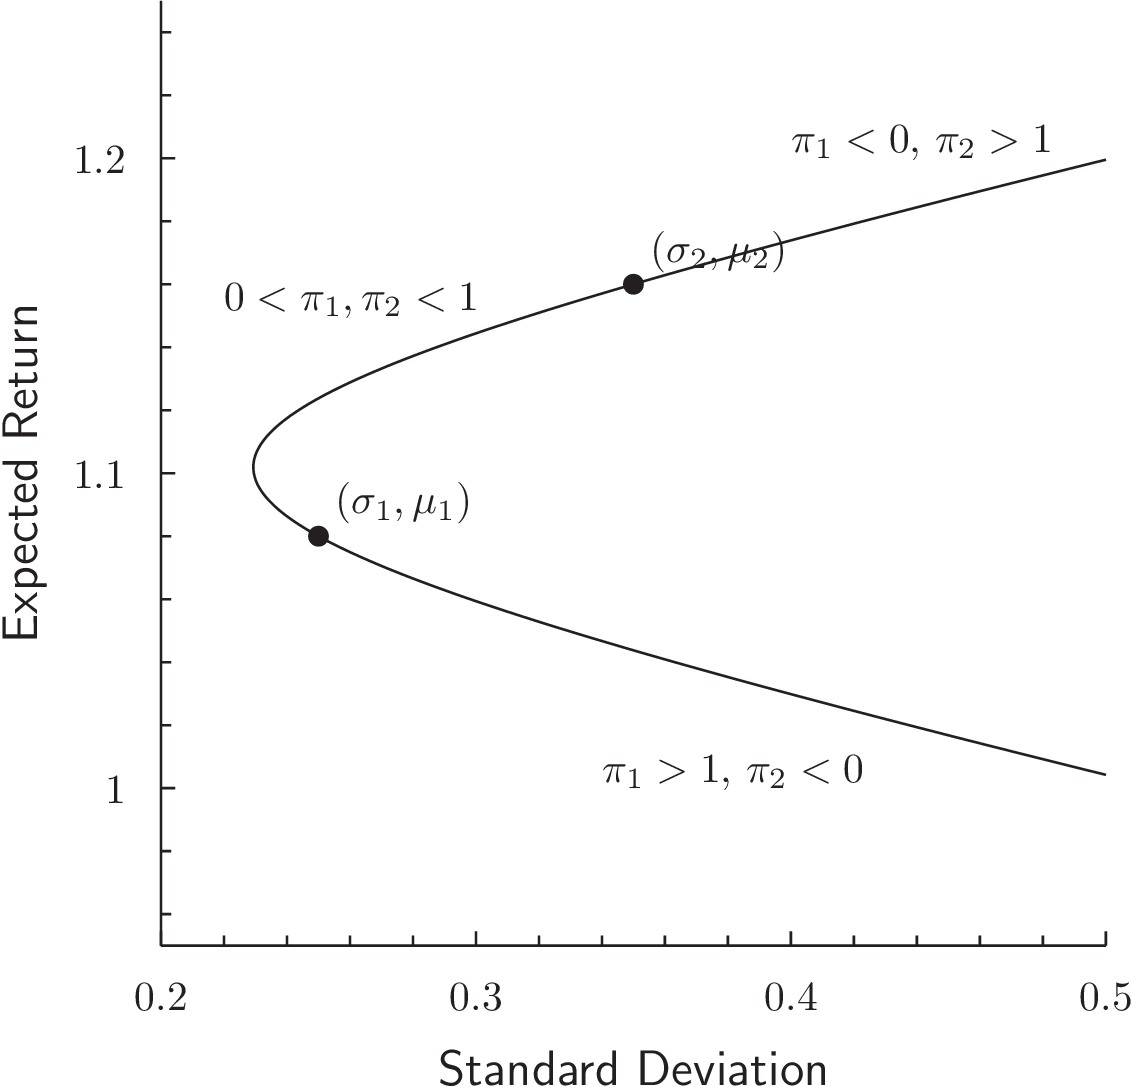
\includegraphics[scale=.7]{Images/fig5_1.png}
  \end{center}
  \vskip -\baselineskip
  \end{frame}
  
  \bfr\frametitle{Portfolios of a Risky and Risk-Free Asset}
  \vskip -\baselineskip
  \begin{center}
  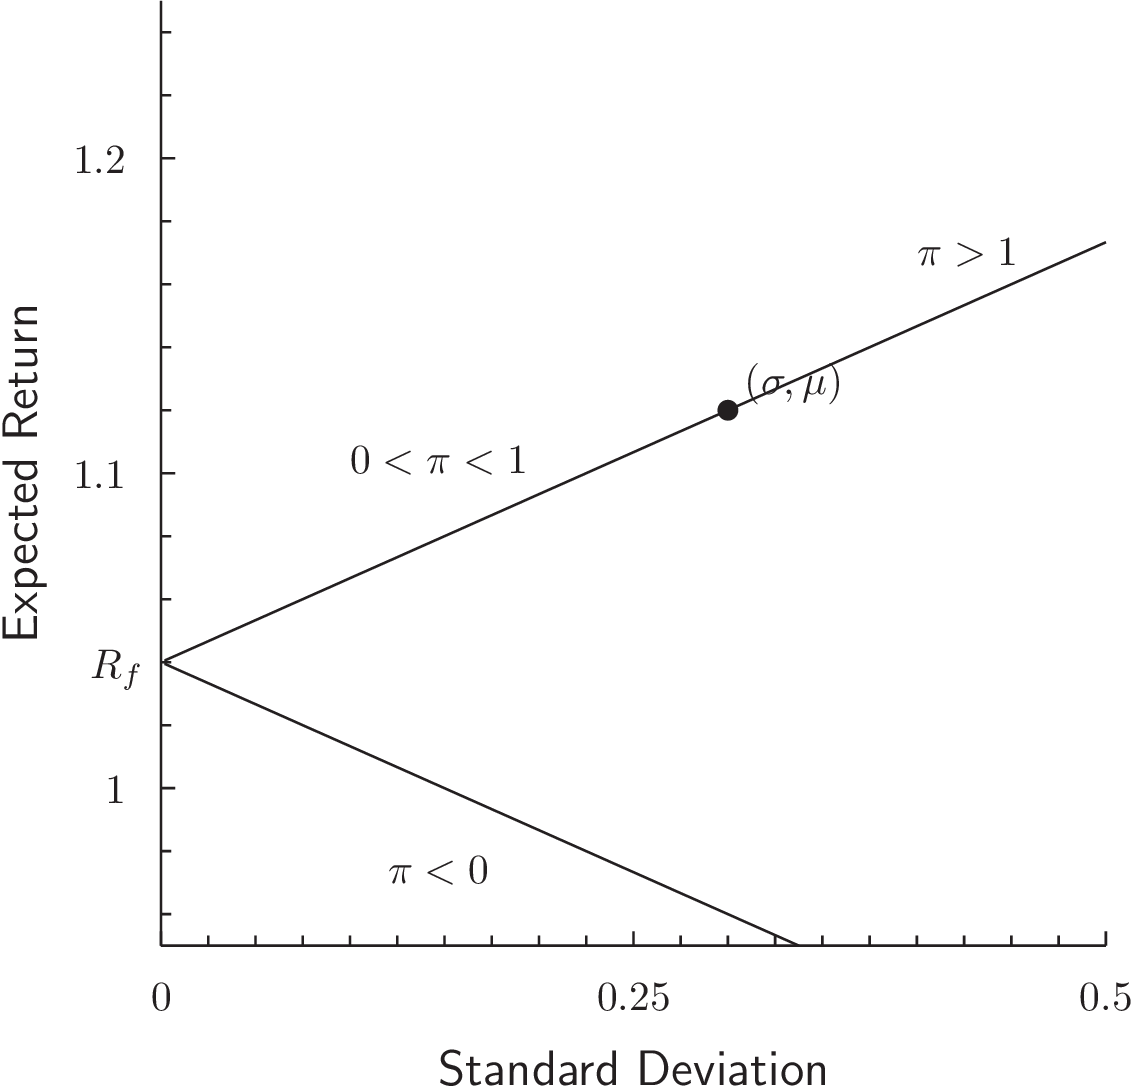
\includegraphics[scale=.7]{Images/fig5_2.png}
  \end{center}
  \vskip -\baselineskip
  \end{frame}
  
  \section{GMV Portfolio}\subsection{}
  
  \bfr\frametitle{Global Minimum Variance Portfolio}
  \bi 
  \im The portfolio of risky assets with minimum variance is called the Global Minimum Variance (GMV) portfolio.
  
  \im It solves the optimization problem
  $$\min \quad\frac{1}{2}\pi'\Sigma\pi \quad\text{subject to}\quad \iota '\pi = 1$$
  \im The Lagrangean for this problem is
  $$\frac{1}{2}\pi'\Sigma\pi - \gamma (\iota '\pi - 1)$$
  \im The FOC is
  $$\Sigma\pi =  \gamma \iota \quad \Leftrightarrow \quad \pi = \gamma\Sigma^{-1}\iota$$
  \im Impose the constraint $\iota '\pi = 1$ and solve for $\gamma$ to obtain
  $$\pi = \frac{1}{\iota ' \Sigma^{-1}\iota} \Sigma^{-1}\iota$$
  \im In other words, take the vector $\Sigma^{-1}\iota$ and divide by the sum of its elements, so the rescaled vector sums to 1.
  \ei 
\end{frame}
  
  \section{Frontier Portfolios}\subsection{}
  
  
  \bfr\frametitle{Mean-Variance Frontier of Risky Assets}
  \bi 
  \im We continue to look at only risky assets so we continue to require portfolio weights to sum to 1 ($\iota'\pi=1$).
  
  \im A \alert{frontier portfolio} is a portfolio that achieves a target expected return with minimum risk.  
  \im It solves an optimization problem
  $$\min \quad\frac{1}{2}\pi'\Sigma\pi \quad\text{subject to}\quad \mu'\pi=\mu_{\text{targ}}\quad\text{and}\quad \iota '\pi = 1$$
  where $\mu_{\text{targ}}$ denotes the given target expected return.
  
  \im By varying the target expected return, we trace out the frontier.
  \ei 
  \end{frame}
  
  \begin{frame}{Solving for Frontier Portfolios}
    \bi 
  \im The Lagrangean for the optimization problem is 
  $$\frac{1}{2}\pi'\Sigma\pi - \delta(\mu'\pi-\mu_{\text{targ}}) - \gamma (\iota '\pi - 1)$$
  \im The FOC is
  $$\Sigma \pi - \delta \mu - \gamma \iota \ = \ 0\,.$$
  \im The solution is
  $$\pi \ = \ \delta \Sigma^{-1}\mu + \gamma\Sigma^{-1}\iota$$
  \im This means that~$\pi$ is a linear combination of the two vectors $\Sigma^{-1}\mu$ and $\Sigma^{-1}\iota$.  
  \im Use constraints to solve for $\delta$ and $\gamma$. 
  \ei
  \end{frame}
  
  \begin{frame}{More Notation}
  \bi 
  \im Denote the GMV portfolio by $\pi_{\text{gmv}}$.  It is $\Sigma^{-1}\iota$ rescaled to sum to 1:
  $$\pi_{\text{gmv}} \ = \ \frac{1}{\iota\Sigma^{-1}\iota}\Sigma^{-1}\iota$$
  
  \im Let's also rescale the vector $\Sigma^{-1}\mu$ to sum to 1 and call it $\pi_\mu$:
  $$\pi_\mu \ = \ \frac{1}{\iota\Sigma^{-1}\mu}\Sigma^{-1}\mu$$
  
  \im To simplify, 
  define
  $A = \mu'\Sigma^{-1}\mu$, $ B = \mu'\Sigma^{-1}\iota$, and $C = \iota '\Sigma^{-1}\iota$.  
  \im Then,
  \begin{align*}
  \pi_{\text{gmv}} \ & = \ \frac{1}{C}\Sigma^{-1}\iota\\
  \pi_\mu \ & = \ \frac{1}{B}\Sigma^{-1}\mu
  \end{align*}
  \ei
  \end{frame}
  
  \begin{frame}{Solution of Frontier Portfolio}
    \bi 
  \im We saw that a frontier portfolio is
  $$\pi = \delta \Sigma^{-1}\mu + \gamma\Sigma^{-1}\iota$$
  for some $\delta$ and $\gamma$.  
  \im We can write this as
  \begin{align*}
  \pi \ &= \ \delta B \frac{1}{B}\Sigma^{-1}\mu + \gamma C \frac{1}{C}\Sigma^{-1}\mu\\
  \ &= \ \delta B \pi_\mu + \gamma C \pi_{\text{gmv}}
  \end{align*}
  \im The constraint $\iota'\pi=1$ implies 
  $$\delta B + \gamma C \ = 1$$
  \im Set $\lambda = \delta B$.  Then, $\gamma C = 1-\lambda$, so the frontier portfolio is 
  $$\pi = \lambda \pi_\mu + (1-\lambda)\pi_{\text{gmv}}$$
  \ei
  \end{frame}
  
  \begin{frame}[plain]
    \bi 
    \im To find the particular frontier portfolio meeting the target return constraint, we can calculate
  $$\mu'\pi = \lambda \mu'\pi_\mu + (1-\lambda) \mu'\pi_{\text{gmv}} \ = \ \lambda \frac{A}{B} + (1-\lambda)\frac{B}{C}$$ 
  \im Set this equal to $\mu_{\text{targ}}$ to obtain
  $$\lambda \ = \ \frac{\mu_{\text{targ}} - B/C}{A/B - B/C} \ = \ \frac{BC\mu_{\text{targ}} - B^2}{AC - B^2}$$
  \ei 
  \end{frame}
  
  \section{Two Fund Spanning}\subsection{}
  \bfr\frametitle{Two Fund Spanning}
  \bi 
  \im The characterization $\pi = \lambda \pi_\mu + (1-\lambda)\pi_{\text{gmv}}$ means that $\pi$ lies on the line through $\pi_\mu$ and $\pi_{\text{gmv}}$ in $\myreal^n$.  
  \im Every frontier portfolio is a combination of $\pi_\mu$ and $\pi_{\text{gmv}}$.  We say that these two portfolios span the frontier.
  
  \im We can consider the portfolios to be funds -- like mutual funds.  If you want a frontier portfolio, you can just invest in these two funds.  We call this two-fund spanning.
  
  \im Any other two points on the line also span the line.  So, any two frontier portfolios can serve as the funds.
  \ei
  \end{frame}
  
\section{Risk-Free Asset}\subsection{}

\bfr\frametitle{Mean-Variance Frontier with a Risk-Free Asset}
\bi 
\im Now, we add a risk-free asset.  We continue to let $\pi\in \myreal^n$ denote the portfolio of risky assets.  
\im We no longer require $\iota'\pi=1$.  The weight on the risk-free asset is $1-\iota'\pi$.  This can be negative (borrowing).
\im 
A portfolio's expected return is
$$(1-\iota'\pi)R_f + \mu'\pi \ = \ R_f + (\mu-R_f\iota)'\pi$$
\im A frontier portfolio solves the following for some $\mu_{\text{targ}}$:
$$\min \quad\frac{1}{2}\pi'\Sigma\pi \quad\text{subject to}\quad R_f + (\mu-R_f\iota )'\pi=\mu_{\text{targ}}$$
\ei
\end{frame}

\begin{frame}
    \bi
 \im FOC is
$$\Sigma\pi - \delta (\mu-R_f\iota ) = 0 \quad \Leftrightarrow \quad \pi = \delta\Sigma^{-1}(\mu-R_f\iota )$$
\im So, all frontier portfolios are scalar multiples of the vector $\Sigma^{-1}(\mu-R_f\iota )$.

\im In other words, the frontier portfolios form a line through the origin and the vector $\Sigma^{-1}(\mu-R_f\iota )$. 
\ei
\end{frame}

\begin{frame}{Tangency Portfolio}
\bi 
\im We can probably divide the vector $\Sigma^{-1}(\mu-R_f\iota )$ by the sum of its elements to form a portfolio of purely risky assets (satisfying $\iota'\pi=1$).  

\im We can do that as long as the sum is nonzero.  That is, we need
$$\iota '\Sigma^{-1}(\mu-R_f\iota ) \ \neq \ 0$$
\im This expression is $B - R_fC$.  It is nonzero if and only if $B/C \neq R_f$.  
\ei 
\end{frame}
\begin{frame}[plain]
    \bi
\im The term $B/C$ is the expected return of the GMV portfolio:
$$\mu'\pi_{\text{gmv}} \ = \ \mu'\left(\frac{1}{\iota'\Sigma^{-1}\iota}\Sigma^{-1}\iota\right) \ = \ \frac{1}{\iota'\Sigma^{-1}\iota}\mu'\Sigma^{-1}\iota \ = \ \frac{B}{C}$$

\im So, when the expected return of the GMV portfolio is different from $R_f$, we 
 can define
 $$
\pi_{\text{tang}} \ = \ \frac{1}{\iota '\Sigma^{-1}(\mu-R_f\iota )}\Sigma^{-1}(\mu-R_f\iota )
$$
\ei 
\end{frame}

\begin{frame}
    \bi 
    \im 
We call this the tangency portfolio because it is on two frontiers: the frontier including the risk-free asset and the frontier of only risky assets.

\im How do we know it is on the frontier of only risky assets?
\begin{enumerate}
\item It is a portfolio constructed from the two vectors $\Sigma^{-1}\mu$ and $\Sigma^{-1}\iota$.
\item Also, anything that solves a less constrained optimization problem (not requiring $\iota'\pi=1$) and satisfies the constraints of a more constrained problem (satisfies $\iota'\pi=1$ anyway) must solve the more constrained problem too.
\end{enumerate}

\im Thus, the two frontiers (in std dev/mean space) must be tangent at this point.
\ei
\end{frame}

\bfr\frametitle{Mean-Variance Frontier: $B/C > R_f$}
\vskip -\baselineskip
\begin{center}
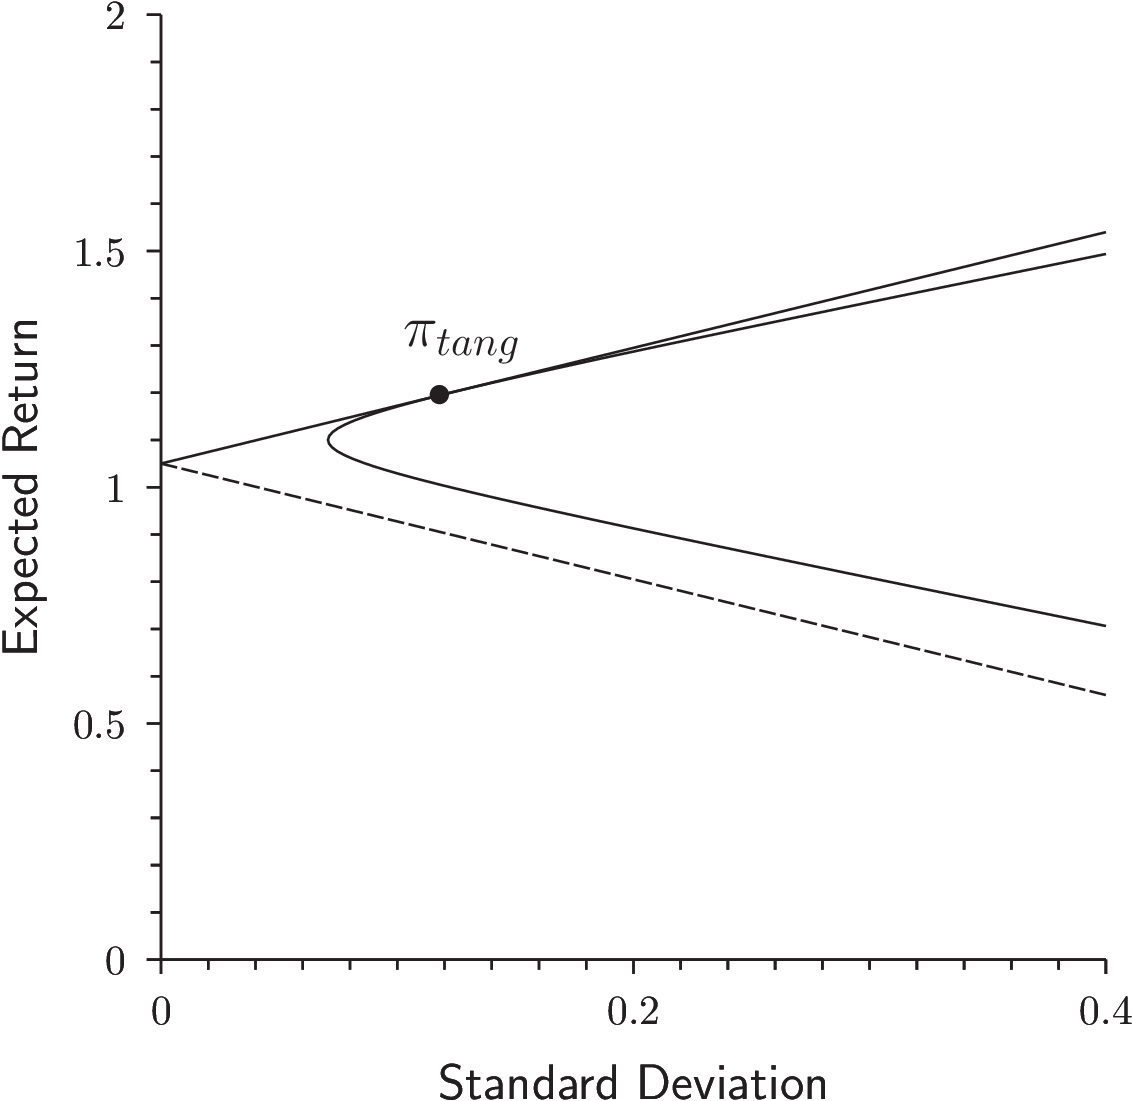
\includegraphics[scale=.7]{images/fig5_3.png}
\end{center}
\vskip -\baselineskip
\end{frame}

\bfr\frametitle{Mean-Variance Frontier: $B/C < R_f$}
\vskip -\baselineskip
\begin{center}
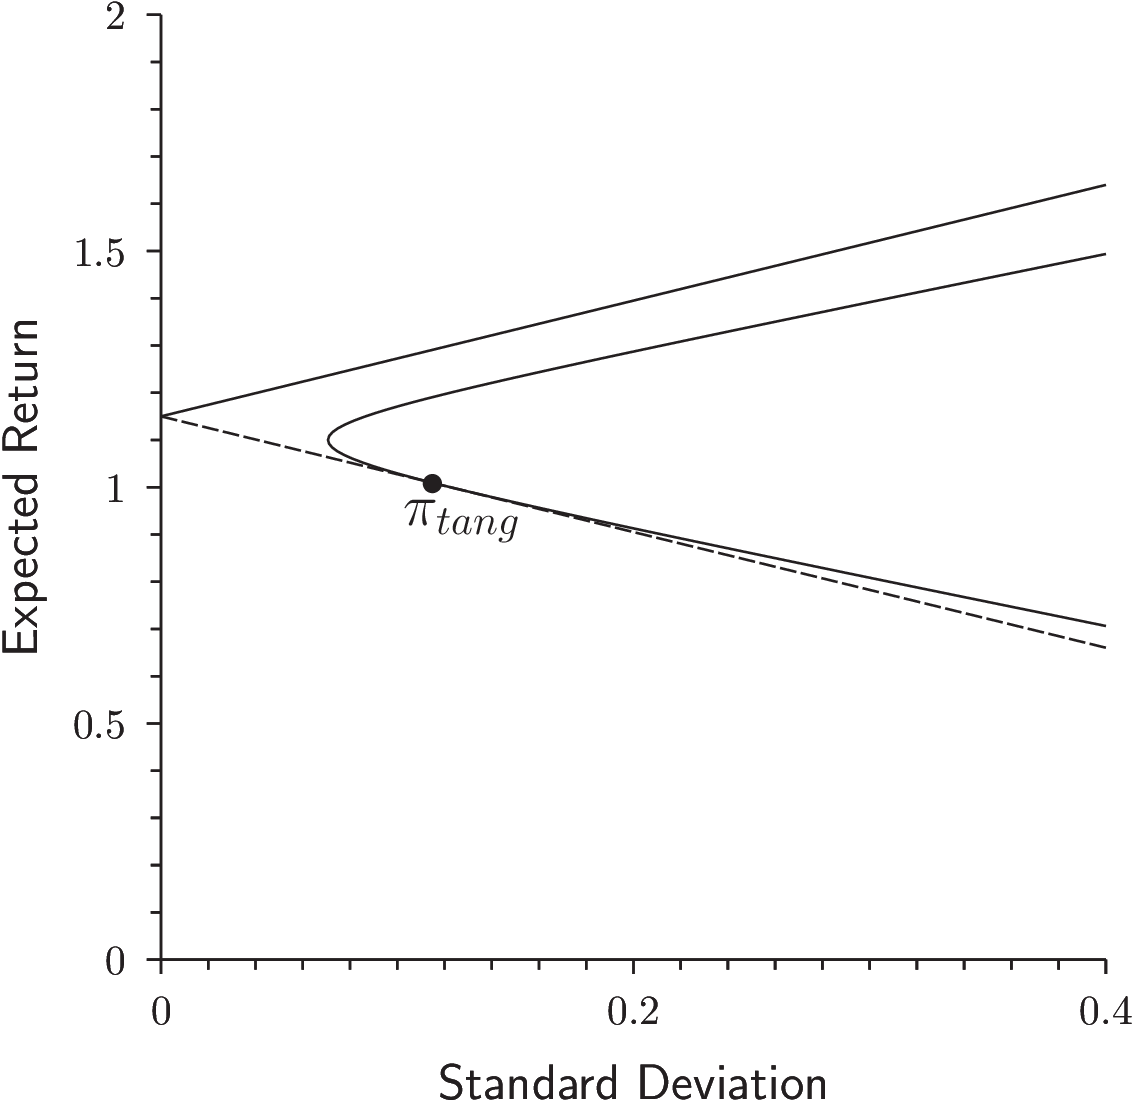
\includegraphics[scale=.7]{images/fig5_4.png}
\end{center}
\vskip -\baselineskip
\end{frame}

\begin{frame}{What if $B/C = R_f$?}
\bi 
\im If $B/C = R_f$, then
\bi 
\im The weights of each frontier portfolio sum to zero.
\im This means investing 100\% in the risk-free asset and then go long and short equal dollars worth of risky assets.
\ei

\im The cone and hyperbola never touch.
\ei
\end{frame}

\section{Two-Fund Spanning Again}
\subsection{}

\bfr\frametitle{Two Fund Spanning with a Risk-Free Asset}
\bi 
\im All frontier portfolios lie on the line through the origin and the vector $\Sigma^{-1}(\mu-R_f\iota)$ in $\myreal^n$.

\im Any vector on the line is a portfolio, because we are not requiring $\iota'\pi=1$.

\im The origin represents 100\% in the risk-free asset.

\im Any two portfolios on the line span the frontier in the sense that any frontier portfolio is a combination $\lambda$ and $(1-\lambda$ of the portfolios.
\ei
\end{frame}

\section{Maximum Sharpe Ratio}
\subsection{}
\begin{frame}{Maximum Sharpe Ratio}
\bi 
\im What is the risk premium of the portfolio $\Sigma^{-1}(\mu-R_f\iota)$?

\im What is the variance of the return of the portfolio $\Sigma^{-1}(\mu-R_f\iota)$?

\im What is its Sharpe ratio (risk premium divided by standard deviation)?
\ei 
\end{frame}



\section{SDFs and Mean-Variance Efficiency}\subsection{}




\begin{frame}[plain]
\bi 
\im Project any SDF onto the span of the assets.  There is a unique projection, and it is an SDF.  Call it $\tm_p$.

\im $\tm_p$ is the payoff of some portfolio (that's what it means to be in the span of the assets).

\im Set $\tr_p = \tm_p / \mye[\tm_p^2]$.  This is $\tm_p$ divided by its cost, so it has a cost of 1 and is a return.  
\im The return $\tr_p$ is an inefficient frontier return.
\im If there is a risk-free asset, then for any frontier return $\tr$, $\tr_p = \lambda R_f + (1-\lambda) \tr$ for some $\lambda$ (by two-fund spanning). So, $\tm_p = a + b\tr$, where $a=\lambda \mye[\tm_p^2]$ and $b = (1-\lambda)\mye[\tm_p^2]$. 
\im Even without a risk-free asset (with one trivial exception), 
\bi
\im SDF = affine function of return $\Rightarrow$ return is on MV frontier.
\im return $\tr$ on MV frontier $\Rightarrow$ $\tm_p = a + b \tr$.
\ei
\ei
\end{frame}

\end{document}
\bfr\frametitle{HJ Bound with a Risk-Free Asset}
For any SDF $\tm$ and any return $\tr$,
$$\frac{\stdev(\tilde{m})}{\mye[\tilde{m}]}\geq  \frac{\stdev(\tilde{m}_p)}{\mye[\tilde{m}_p]} \geq  \frac{|\mye[\tilde{R}]-R_f|}{\stdev(\tilde{R})}$$
The right-hand side is the absolute value of the Sharpe ratio of $\tr$.

The second inequality is an equality for the maximum Sharpe ratio.  In fact, $$ \frac{\stdev(\tilde{m}_p)}{\mye[\tilde{m}_p]} = \frac{|\mye[\tilde{R}_p]-R_f|}{\stdev(\tilde{R}_p)}$$

\end{frame}

\section{Risk Premia}\subsection{}

\bfr\frametitle{The FOC with a Risk-Free Asset}
The FOC for the frontier with a risk-free asset is
$$\Sigma\pi \ = \ \delta (\mu-R_f\iota )$$
We solved it for $\pi$:
$$ \pi \ = \ \delta\Sigma^{-1}(\mu-R_f\iota )$$
We can instead solve it for the vector of risk premia:
$$\mu - R_f\iota \ = \ \frac{1}{\delta}\Sigma\pi$$
 What is $\Sigma \pi$?
\end{frame}



\end{document}

\end{document}

The constraint
$\mu'\pi = \mu_{\text{targ}}$ implies 
$$\delta BA + \gamma CB \ = \ \mu_{\text{targ}}$$
\im Can solve these two equations in two unknowns for $\delta$ and $\gamma$.